\subsection{Writing beyond array bounds}

OK, we read some values from the stack \IT{illegally}, but what if we could write something to it?

Here is what we have got:

\lstinputlisting{patterns/13_arrays/2_BO/w.c}

\subsubsection{MSVC}

And what we get:

\lstinputlisting[caption=\NonOptimizing MSVC 2008]{patterns/13_arrays/2_BO/w_EN.asm}

The compiled program crashes after running. No wonder. Let's see where exactly does it is crash.

\clearpage
\myindex{\olly}

Let's load it into \olly, and trace until all 30 elements are written:

\begin{figure}[H]
\centering
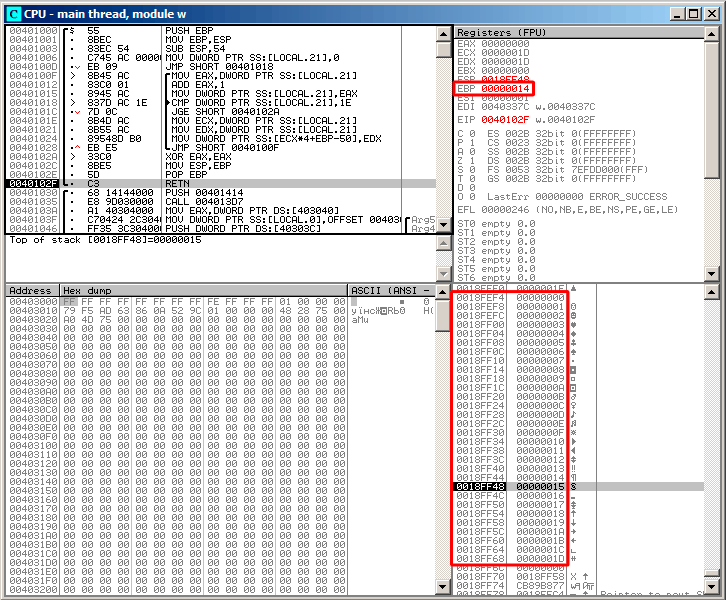
\includegraphics[scale=\FigScale]{patterns/13_arrays/2_BO/olly_w1.png}
\caption{\olly: after restoring the value of EBP}
\label{fig:array_BO_olly_w1}
\end{figure}

\clearpage
Trace until the function end:

\begin{figure}[H]
\centering
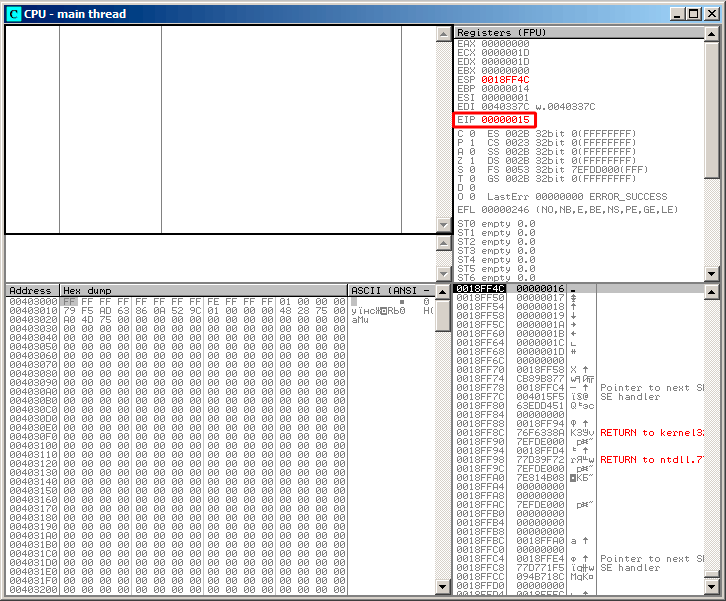
\includegraphics[scale=\FigScale]{patterns/13_arrays/2_BO/olly_w2.png}
\caption{\olly: 
EIP was restored, but \olly can't disassemble at 0x15}
\label{fig:array_BO_olly_w2}
\end{figure}

Now please keep your eyes on the registers.

\EIP is 0x15 now. It is not a legal address for code---at least for win32 code!
We got there somehow against our will.
It is also interesting that the \EBP register contain 0x14,
\ECX and \EDX contain 0x1D.

Let's study stack layout a bit more.

After the control flow was passed to \TT{\main}, the value in the \EBP register was saved on the stack.
Then, 84 bytes were allocated for the array and the $i$ variable.
That's \TT{(20+1)*sizeof(int)}.
\ESP now points to the \TT{\_i} variable in the local stack and after the execution of 
the next \TT{PUSH something}, \IT{something} is appearing next to \TT{\_i}.

That's the stack layout while the control is in \main:

\begin{center}
\begin{tabular}{ | l | l | }
\hline
  \TT{ESP}    & 4 bytes allocated for $i$ variable \\
\hline
  \TT{ESP+4}  & 80 bytes allocated for \TT{a[20]} array \\
\hline
  \TT{ESP+84} & saved \EBP value \\
\hline
  \TT{ESP+88} & return address \\
\hline
\end{tabular}
\end{center}

\TT{a[19]=something} statement writes the last \Tint in the bounds of the array (in bounds so far!).

\TT{a[20]=something} statement writes \IT{something} to the place where the value of \EBP is saved.

Please take a look at the register state at the moment of the crash. In our case,
20 was written in the 20th element. 
At the function end, the function epilogue restores the original \EBP value.
(20 in decimal is \TT{0x14} in hexadecimal).
Then \RET gets executed, which is effectively equivalent to \TT{POP EIP} instruction.

The \RET instruction takes the return address from the stack (that is the address in \ac{CRT}),
which was called \main),
and 21 iss stored there (\TT{0x15} in hexadecimal).
The CPU traps at address \TT{0x15},
but there is no executable code there, so exception gets raised.

\myindex{\BufferOverflow}

Welcome! It is called a \IT{buffer overflow}\footnote{\href{http://go.yurichev.com/17132}{wikipedia}}.

Replace the \Tint array with a string (\Tchar array), create a long string deliberately
and pass it to the program, to the function, which doesn't check the length of the string and copies it in a short buffer,
and you'll able to point the program to an address to which it must jump.
It's not that simple in reality, but that is how it emerged.
Classic article about it: \AlephOne.

\subsubsection{GCC}

Let's try the same code in GCC 4.4.1. We get:

\lstinputlisting{patterns/13_arrays/2_BO/w_gcc.asm}

Running this in Linux will produce: \TT{Segmentation fault}.

\myindex{GDB}

If we run this in the GDB debugger, we get this:

\begin{lstlisting}
(gdb) r
Starting program: /home/dennis/RE/1 

Program received signal SIGSEGV, Segmentation fault.
0x00000016 in ?? ()
(gdb) info registers
eax            0x0	0
ecx            0xd2f96388	-755407992
edx            0x1d	29
ebx            0x26eff4	2551796
esp            0xbffff4b0	0xbffff4b0
ebp            0x15	0x15
esi            0x0	0
edi            0x0	0
eip            0x16	0x16
eflags         0x10202	[ IF RF ]
cs             0x73	115
ss             0x7b	123
ds             0x7b	123
es             0x7b	123
fs             0x0	0
gs             0x33	51
(gdb) 
\end{lstlisting}

The register values are slightly different than in win32 example, 
since the stack layout is slightly different too.

